\section{Background}
John Maynard Keynes work revolutionized economic thought; however, he never formalized any of his theories into a mathematical theory. This was done over several decades in a process known as the Neo-classical synthesis which sought to connect traditional, classical models with newer Keynesian ideas\autocite{Fazzari1989}. In 1939, Paul Samuelson developed a popular model that could display endogenous, business-cycle behavior which married Keynes' investment multiplier theory with Clarke's accelerator principle\autocite{Puu2003,Press1939}.

The model is often criticized for the amount of simplifying assumptions it makes for the sake of mathematical simplicity. It is for this reason that later models feature significantly more mechanisms at play; however, this model is still useful for studying how cyclic behavior can be derived endogenously purely through economic fundamentals.
\subsection{Accelerator Theory and Investment}
Key to the idea of the accelerator effect is that growth has a positive effect on the level of investment. Economic growth features an overall increase in business profits and business confidence, thereby resulting in increases in fixed investments to grow business further. However, a recession decreases business profits and confidence and damages their ability and willingness to invest for the future. 

Earlier implementations of this theory used a simple, linear function to represent the relationship between investment and income. This however, was questioned on its applicability to real world behavior as it implied that business actively destroyed preexisting investments if income declined faster than the natural rate of capital depreciation. In the 1950s, Hicks suggested a linear, piecewise function with upper and lower bounds\autocite{Puu2003}. The lower bound represented the natural rate of capital depreciation thereby giving a minimal level of investment loss. The upper bound was rationalized to be a result of decreasing marginal gains to productivity from investment as land, labor, and raw materials became limiting factors to production. 

Richard Goodwin found a different solution in the form of a hyperbolic tangent function that asymptotically approached the limits of the piecewise function. This function was differentiable at all points which allows us to derive the form of the function used for our multiplier-accelerator model. Our investment function is a linear-cubic taylor series expansion of the hyperbolic tangent function which introduces a fundamental change in the function by causing it to backbend to 0 instead of asymptotically approaching a non-zero limit. This can be rationalized by introducing counter-cyclic government economic policy. During a recession, governments will increase spending in an attempt to counteract market behavior and stimulate the economy. Likewise, governments will take advantage of expansionary periods by increasing taxes and reducing government projects relative to recessionary periods allowing the government to possess the necessary funds to sustain investments come the next recessionary period. Our investment function can thus be thought of as being representative of both public and private investments.\autocite{Puu2003}

Investments are thus treated as a function of the change in income in the past with lag introduced, making it a second-order difference equation of the linear-cubic form:
\begin{equation}
    I_t=\mu(Y_{t-1}-Y_{t-2})-\mu(Y_{t-1}-Y_{t-2})^3
\end{equation}
\subsection{The Keynesian Multiplier and Consumption}
\section{Stability and Chaos in Income Dynamics}

\begin{figure}
    \centering
    \includegraphics[width=\textwidth]{./sam_hicks/2-cyclic.pdf}
    \caption{Cyclic growth behavior in the }
\end{figure}
\begin{figure}
    \centering
    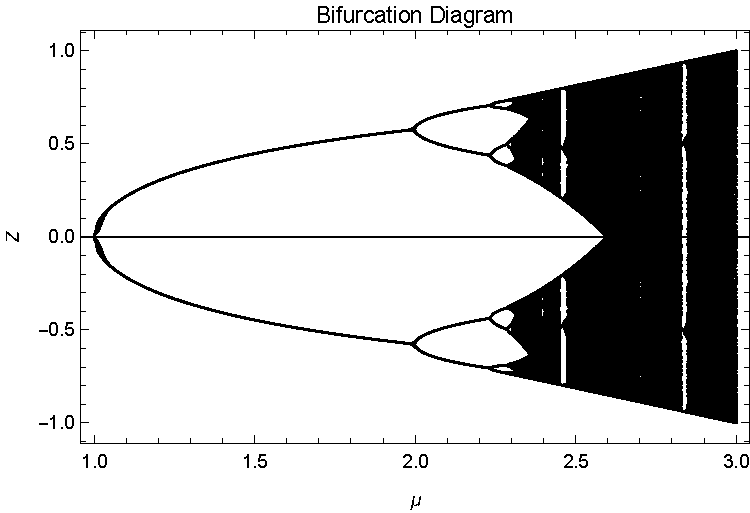
\includegraphics[width=\textwidth]{./sam_hicks/bifurcation.pdf}
    \caption{Bifurcation diagram of samuelson-hicks model. Plot overlays bifurcation diagram with intial value of 0.1 and -0.1 as the mapping prevents from a growth to decay region for all parameter values.}
\end{figure}
\begin{figure}
    \centering
    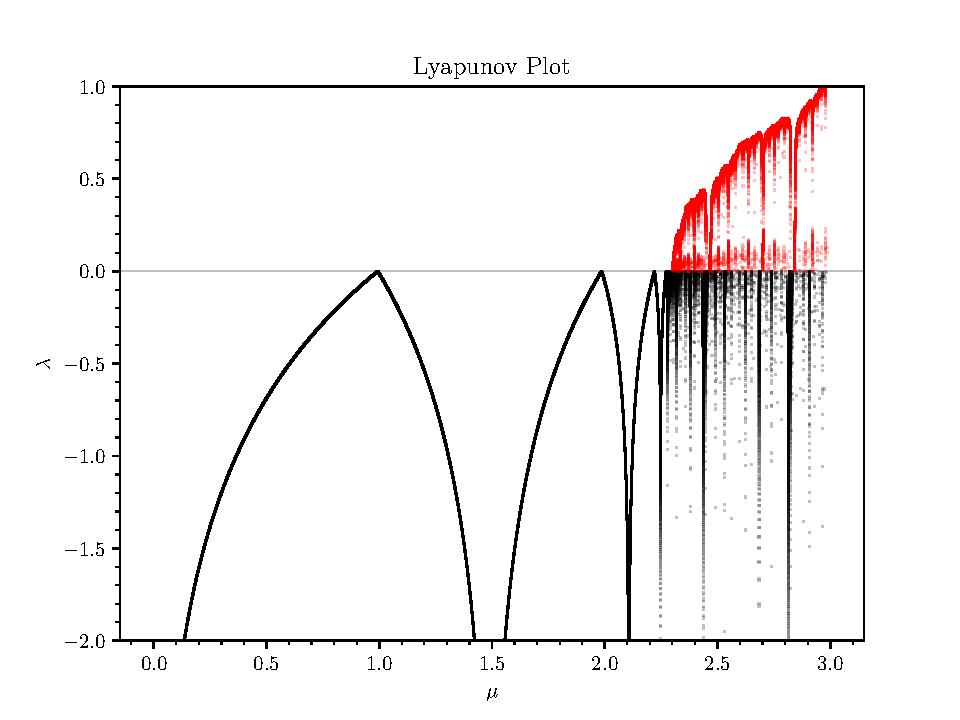
\includegraphics[width=\textwidth]{./sam_hicks/lyapunov.pdf}
    \caption{Lyapunov exponent plotted against $\mu$ for the samuelson-hicks. Initial value set to 0.1. Red denotes regions where $\lambda\geq0$, black denotes regions where $\lambda<0$}
\end{figure}